% Adjust these for the path of the theme and its graphics, relative to this file
%\usepackage{beamerthemeFalmouthGamesAcademy}
\usepackage{../../beamerthemeFalmouthGamesAcademy}
\usepackage{multimedia}
\graphicspath{ {../../} }

% Default language for code listings
\lstset{language=C++,
        morekeywords={each,in,nullptr}
}

% For strikethrough effect
\usepackage[normalem]{ulem}
\usepackage{wasysym}

\usepackage{pdfpages}

% http://www.texample.net/tikz/examples/state-machine/
\usetikzlibrary{arrows,automata}

\newcommand{\modulecode}{COMP260}\newcommand{\moduletitle}{Distributed Systems}\newcommand{\sessionnumber}{5}

\begin{document}
\title{Game Analytics}
\subtitle{\modulecode\ \moduletitle}

\frame{\titlepage}

\begin{frame}{Announcement for BSc first years}
	\begin{itemize}
		\pause\item \textbf{COMP130 Worksheet D} is now live
		\pause\item This is the final worksheet
		\pause\item Assesses your \textbf{individual contribution} to the \textbf{team game}
		\pause\item Minimal extra work for you :)
	\end{itemize}
\end{frame}

\part{What is PCG?}
\frame{\partpage}

\begin{frame}{What is procedural content generation (PCG)?}
	\begin{itemize}
		\item<3-> \textbf{Procedural}: by computer program or algorithm,
			with little or no direct input from designer or user
		\item<2-> \textbf{Content}: levels, maps, art, animations, stories, items,
			quests, music, weapons, vehicles, characters, ...
		\item<1-> \textbf{Generation}: creating stuff
	\end{itemize}
\end{frame}

\begin{frame}{Types of PCG}
	\begin{itemize}
		\pause\item \textbf{Online}
			\begin{itemize}
				\pause\item Generate content at run-time
				\pause\item Part of the game
			\end{itemize}
		\pause\item \textbf{Offline}
			\begin{itemize}
				\pause\item Generate content at design-time
				\pause\item Tool for developers
			\end{itemize}
	\end{itemize}
\end{frame}

\begin{frame}{PCG $\neq$ randomness}
	\begin{itemize}
		\pause\item Many PCG systems use random numbers, but randomness in itself is not PCG
		\pause\item Can have PCG without randomness, e.g.\ based on fractals or simulations
		\pause\item Randomness in PCG is generally \textbf{constrained} to produce desired content
		\pause\item Shuffling a deck of cards for a game of Solitaire is \textbf{not} PCG!
	\end{itemize}
\end{frame}

% \begin{frame}{Not to be confused with...}
% 	\begin{itemize}
% 		\pause\item \textbf{Procedural Rhetoric} / \textbf{Procedurality} (Bogost)
% 		\pause\item ``the art of persuasion through rule-based representations and interactions,
% 			rather than the spoken word, writing, images, or moving pictures''
% 		\pause\item There: ``procedural'' = ``rule-based''
% 		\pause\item Here: ``procedural'' = ``algorithmic''
% 	\end{itemize}
% \end{frame}

\begin{frame}{Why PCG?}
	\begin{itemize}
		\pause\item More content for less development effort
		\pause\item Decrease development costs
		\pause\item Increase replayability
		\pause\item Decrease storage requirements
		\pause\item Allow game mechanics based on unseen content
	\end{itemize}
\end{frame}

\begin{frame}{Further reading}
	Noor Shaker, Julian Togelius and Mark J. Nelson.
	\textit{Procedural Content Generation in Games: A textbook and an overview of current research}.
	Springer, 2016.
	
	Available online: \url{http://pcgbook.com}
\end{frame}

\part{Analysing data}
\frame{\partpage}

\begin{frame}
	\begin{center}
		
\includegraphics[height=0.9\textheight]{science_bitch}
	\end{center}
\end{frame}

\begin{frame}{The scientific method}
	\begin{center}
		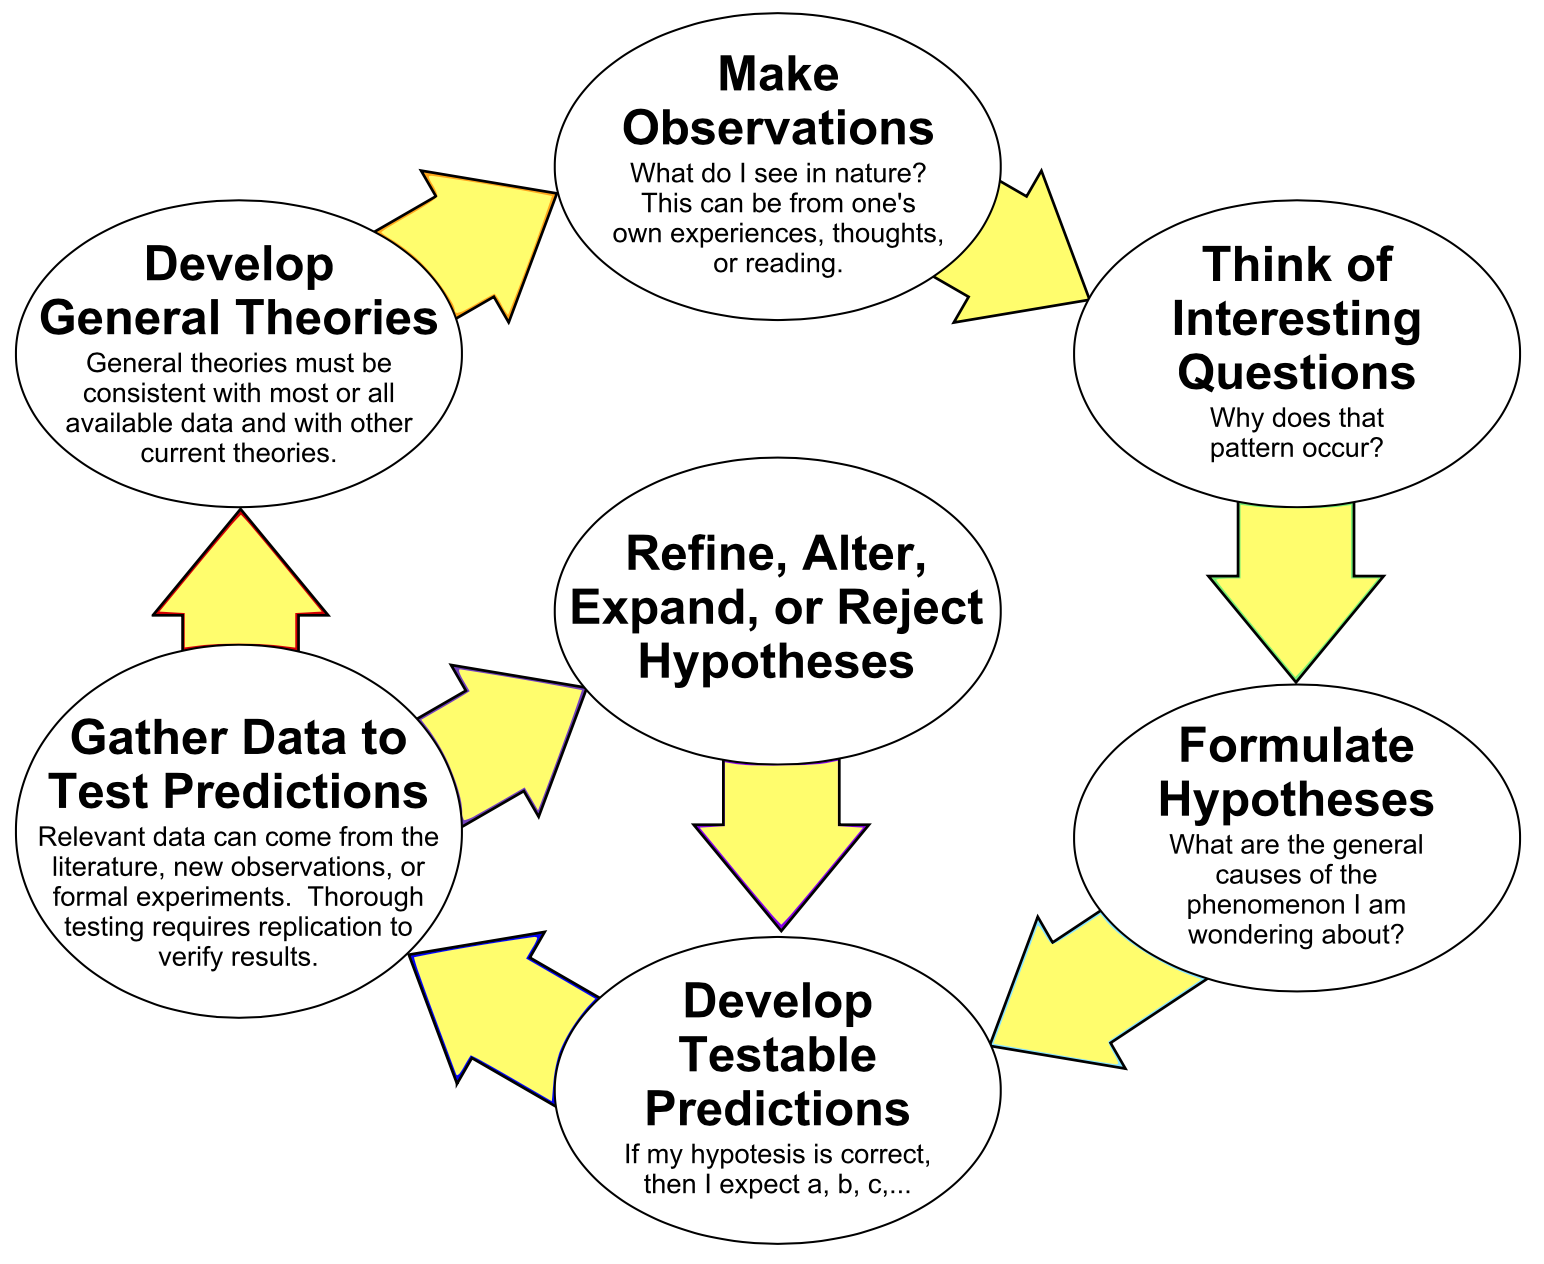
\includegraphics[width=0.8\textwidth]{scientific_method}
	\end{center}
\end{frame}

\begin{frame}{Statistical significance}
	\pause Is a D6 biased if...
	\begin{itemize}
		\pause\item You roll it once and it comes up a six?
		\pause\item You roll it 3 times and it comes up a six twice?
		\pause\item You roll it 60 times and it comes up a six 59 times?
		\pause\item You roll it 60 times and it comes up a six 11 times?
		\pause\item You roll it 600 times and it comes up a six 110 times?
		\pause\item You roll it 6,000,000 times and it comes up a six 1,100,000 times?
	\end{itemize}
\end{frame}

\begin{frame}{Statistical significance}
	\begin{itemize}
		\pause\item Every statistical result has a non-zero probability of being a \textbf{coincidence}
		\pause\item Know your \textbf{confidence intervals}
		\pause\item Beware of \textbf{$p$-value fishing}
	\end{itemize}
\end{frame}

\begin{frame}
	\begin{center}
		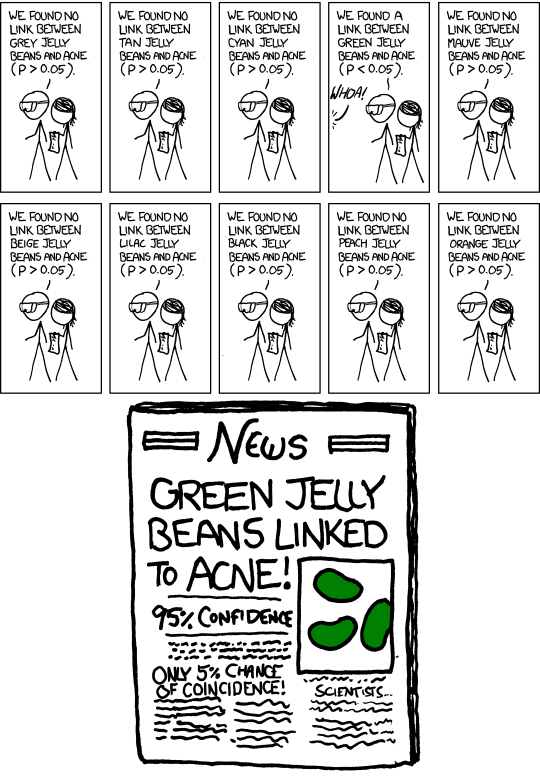
\includegraphics[height=0.9\textheight]{xkcd_significant_crop}
	\end{center}	
\end{frame}

\begin{frame}{Statistical significance vs effect size}
	\begin{itemize}
		\pause\item High statistical significance does not always mean large \textbf{effect size}
		\pause\item E.g.\ red team wins 5,010,000 matches out of 10,000,000
		\pause\item This is statistically significant, but only a 0.1\% effect size
	\end{itemize}
\end{frame}

\begin{frame}{Correlation does not imply causation}
	\pause
	\begin{center}
		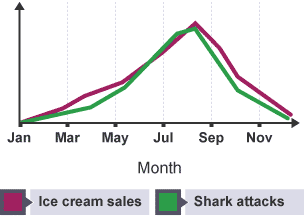
\includegraphics[height=0.5\textheight]{shark_attacks}
	\end{center}
\end{frame}

\begin{frame}{Correlation does not imply causation}
	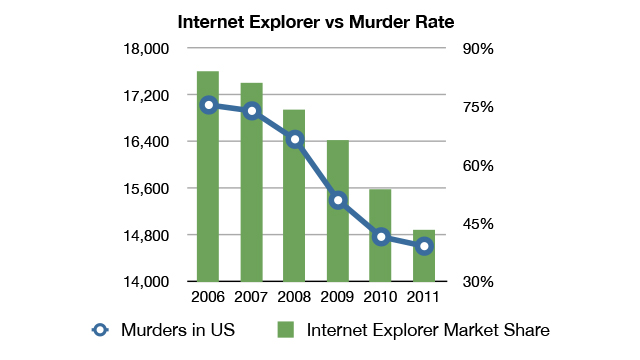
\includegraphics[width=\textwidth]{internet_explorer_murder_rate}
\end{frame}


\part{Data-driven decision making}
\frame{\partpage}

\begin{frame}
	\begin{center}
		
\includegraphics[width=0.6\textwidth]{valve_logo}
		
		\url{https://youtu.be/HQwL6zh7AgA}
		
		\url{http://media.steampowered.com/apps/steamdevdays/slides/data.pdf}
	\end{center}
\end{frame}

\begin{frame}{Decision making at Valve}
	\begin{itemize}
		\pause\item Valve favour \textbf{data-driven decision making}
			\begin{itemize}
				\pause\item Ask \textbf{explicit} questions
				\pause\item Look at the \textbf{data}
				\pause\item Use the data to develop a \textbf{theory}
				\pause\item Define \textbf{measurable outcomes}
				\pause\item \textbf{Iterate}
			\end{itemize}
	\end{itemize}
\end{frame}

\begin{frame}
	\begin{tikzpicture}[remember picture, overlay]
		\node[at=(current page.center)] {
			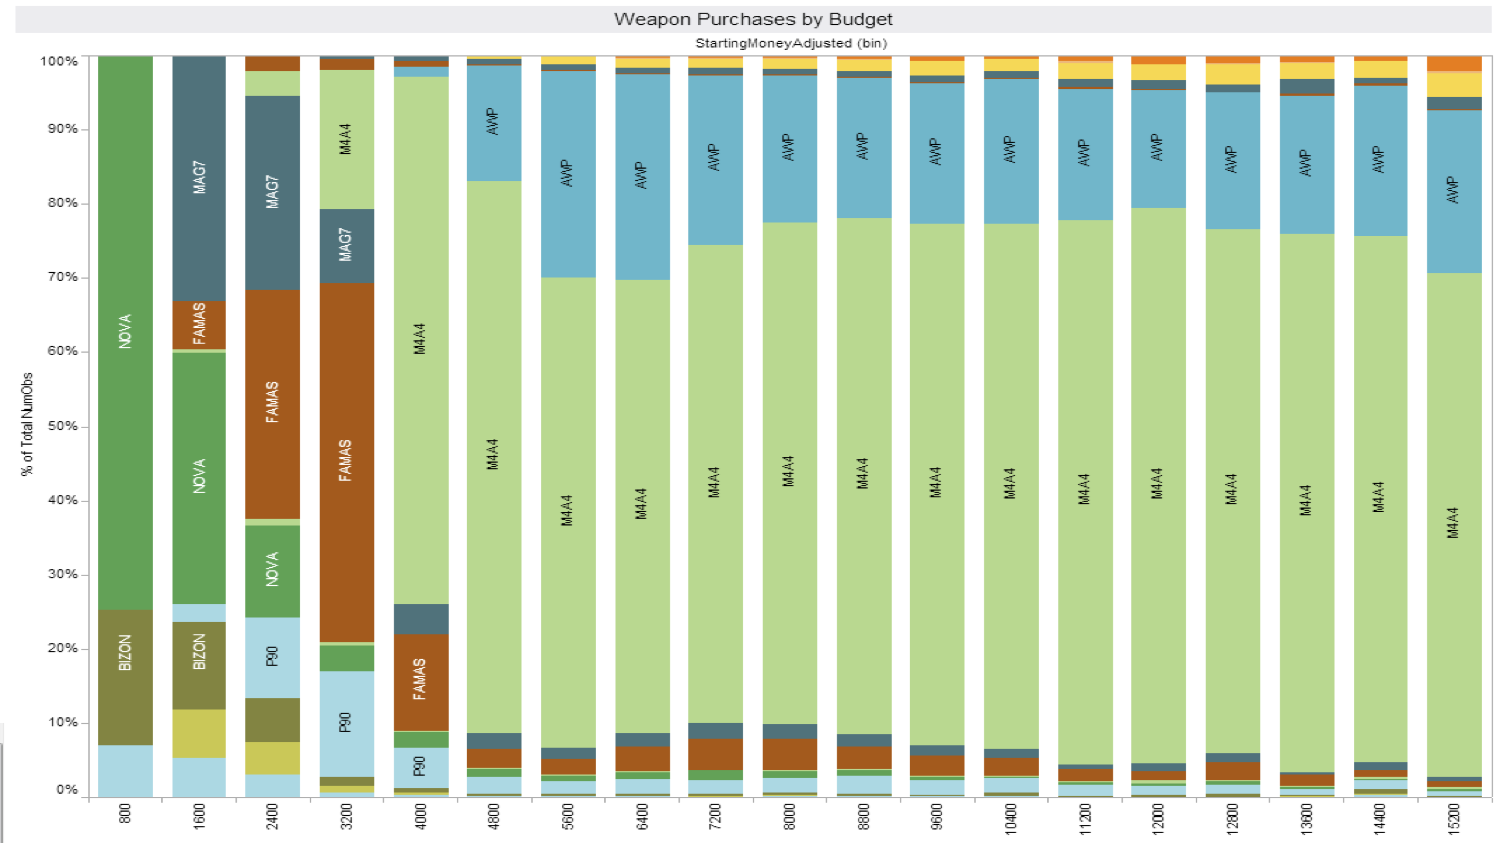
\includegraphics[width=\paperwidth]{csgo_1}
		};
	\end{tikzpicture}
\end{frame}

\begin{frame}
	\begin{tikzpicture}[remember picture, overlay]
		\node[at=(current page.center)] {
			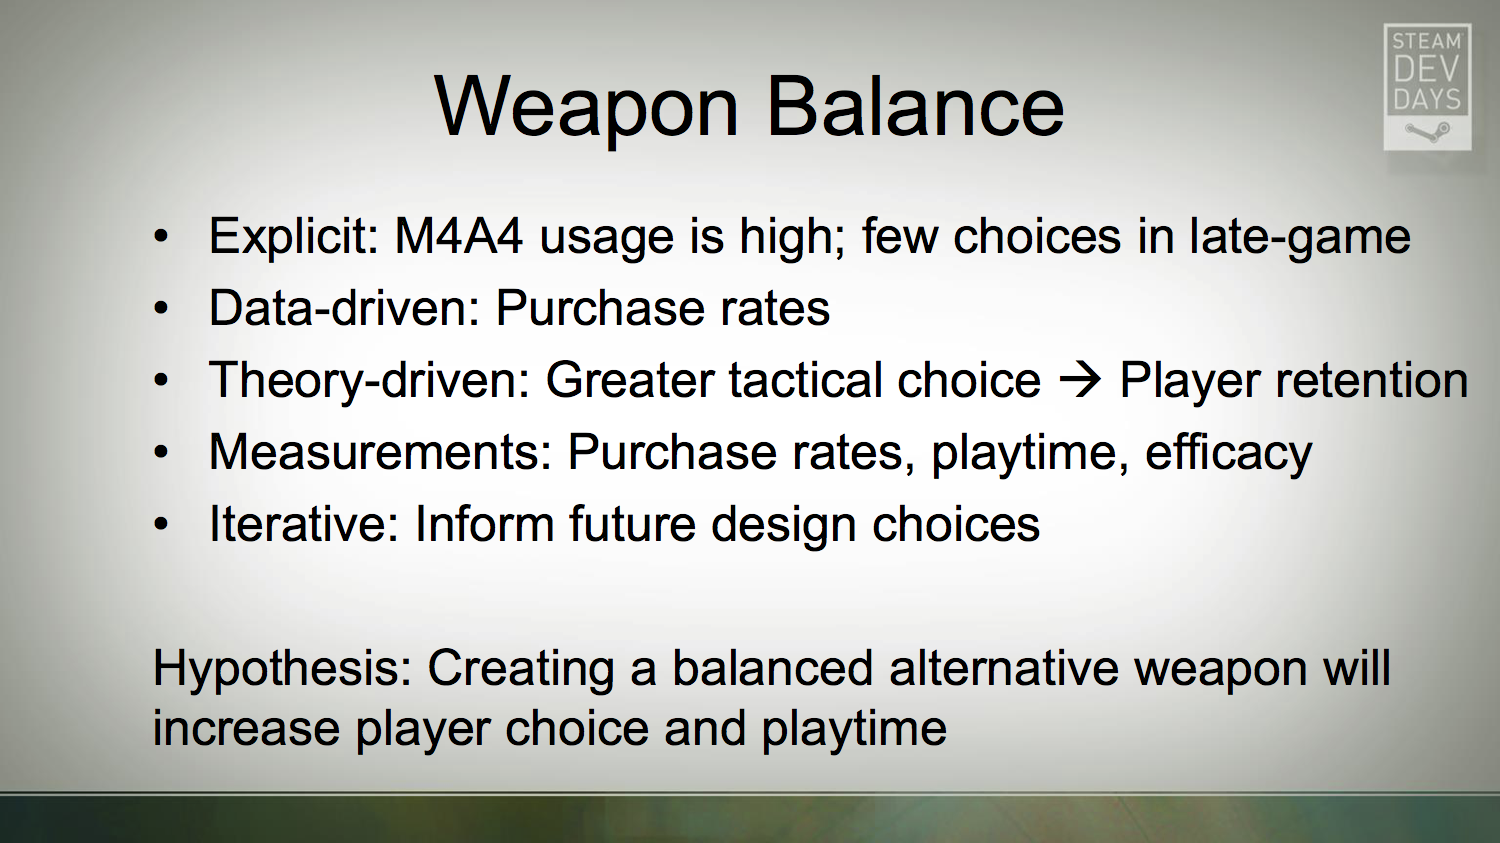
\includegraphics[width=\paperwidth]{csgo_2}
		};
	\end{tikzpicture}
\end{frame}

\begin{frame}
	\begin{tikzpicture}[remember picture, overlay]
		\node[at=(current page.center)] {
			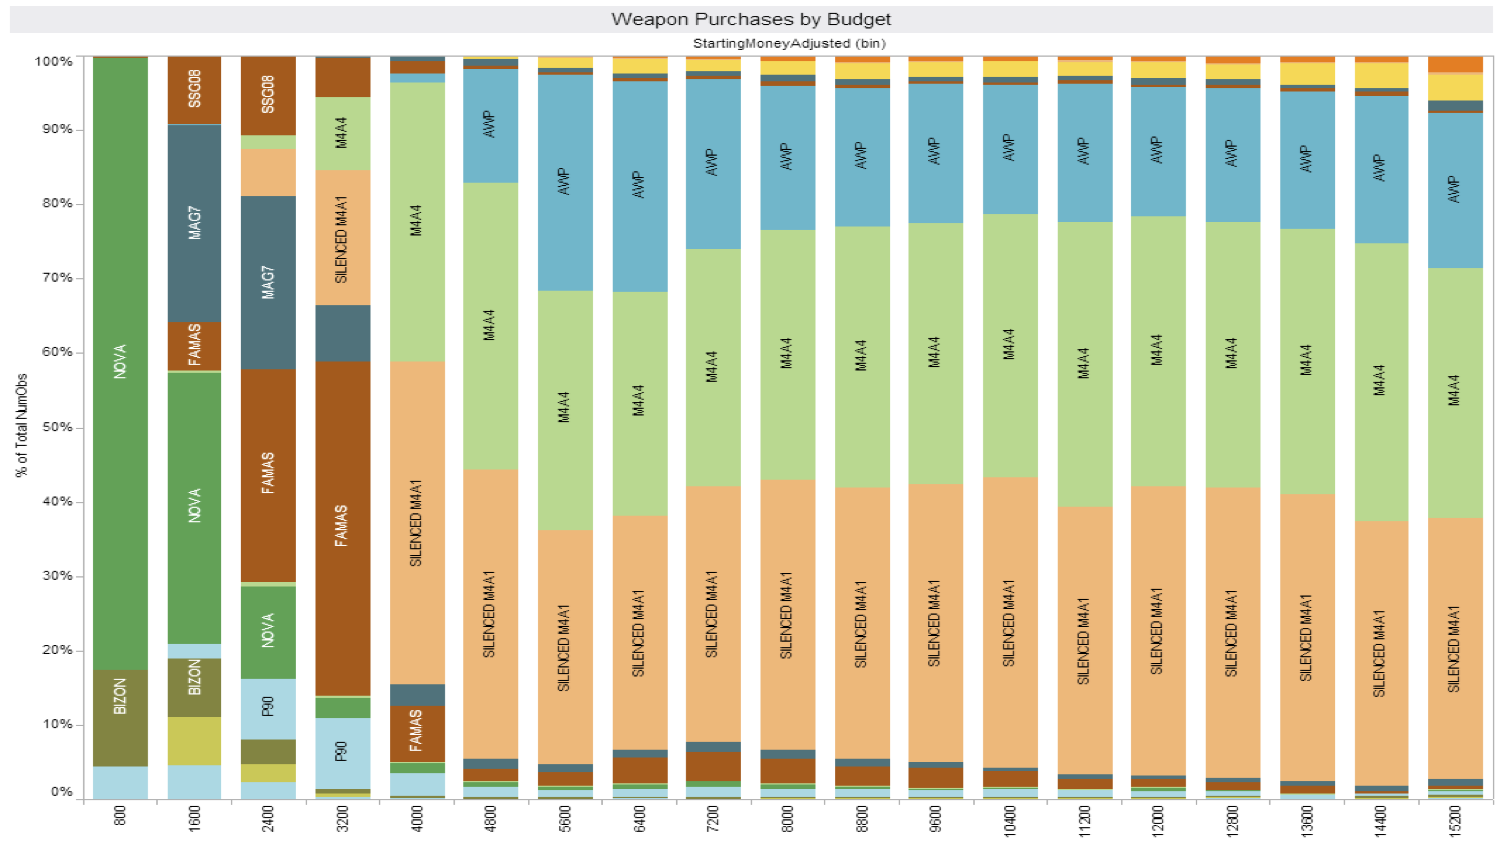
\includegraphics[width=\paperwidth]{csgo_3}
		};
	\end{tikzpicture}
\end{frame}

\begin{frame}
	\begin{tikzpicture}[remember picture, overlay]
		\node[at=(current page.center)] {
			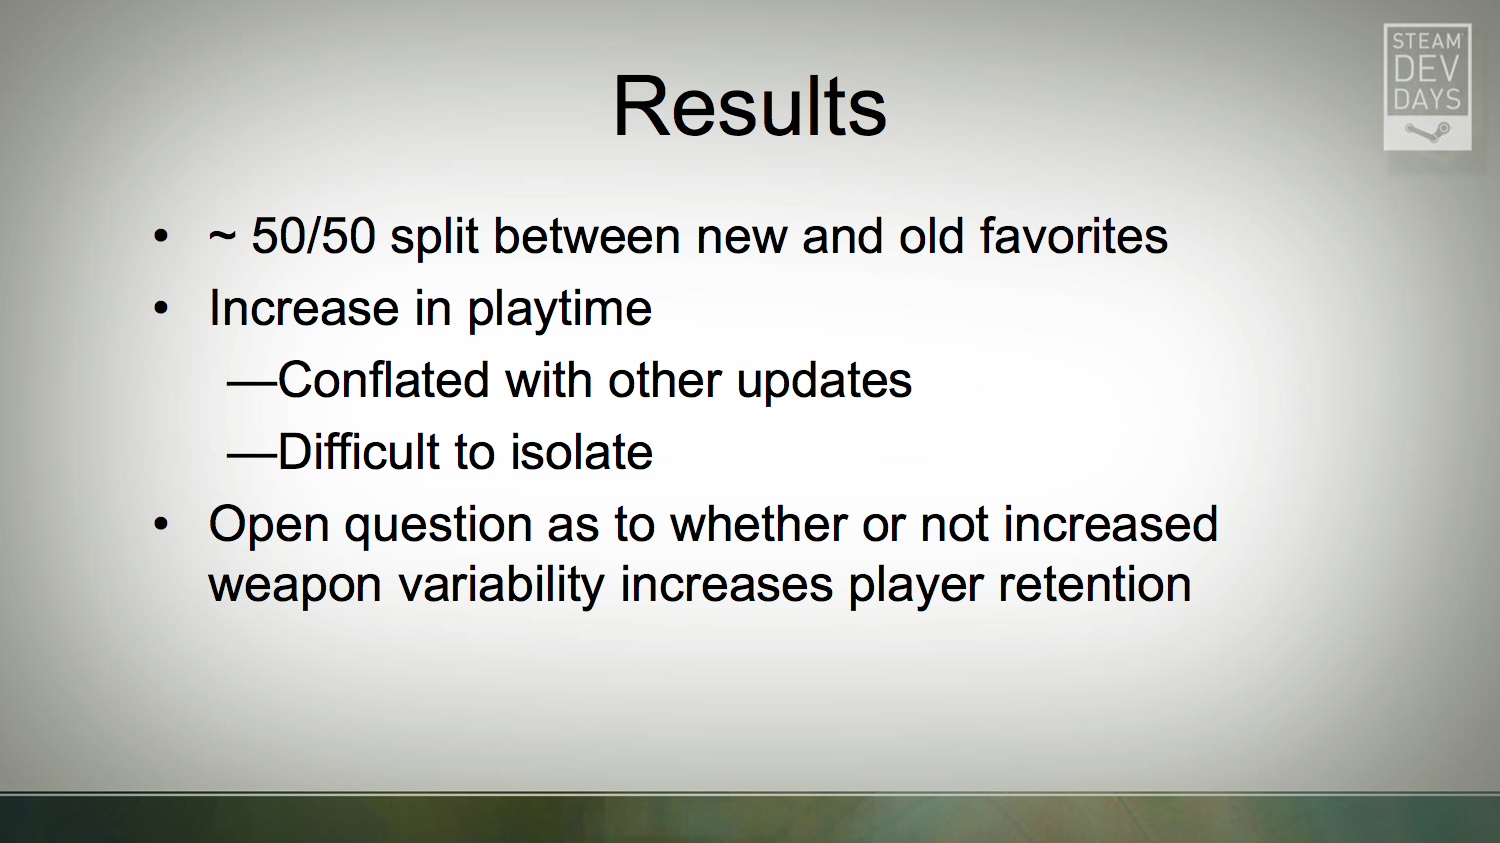
\includegraphics[width=\paperwidth]{csgo_4}
		};
	\end{tikzpicture}
\end{frame}

\begin{frame}{Data visualisation}
	\begin{tikzpicture}[remember picture, overlay]
		\node[at=(current page.south), anchor=south] {
			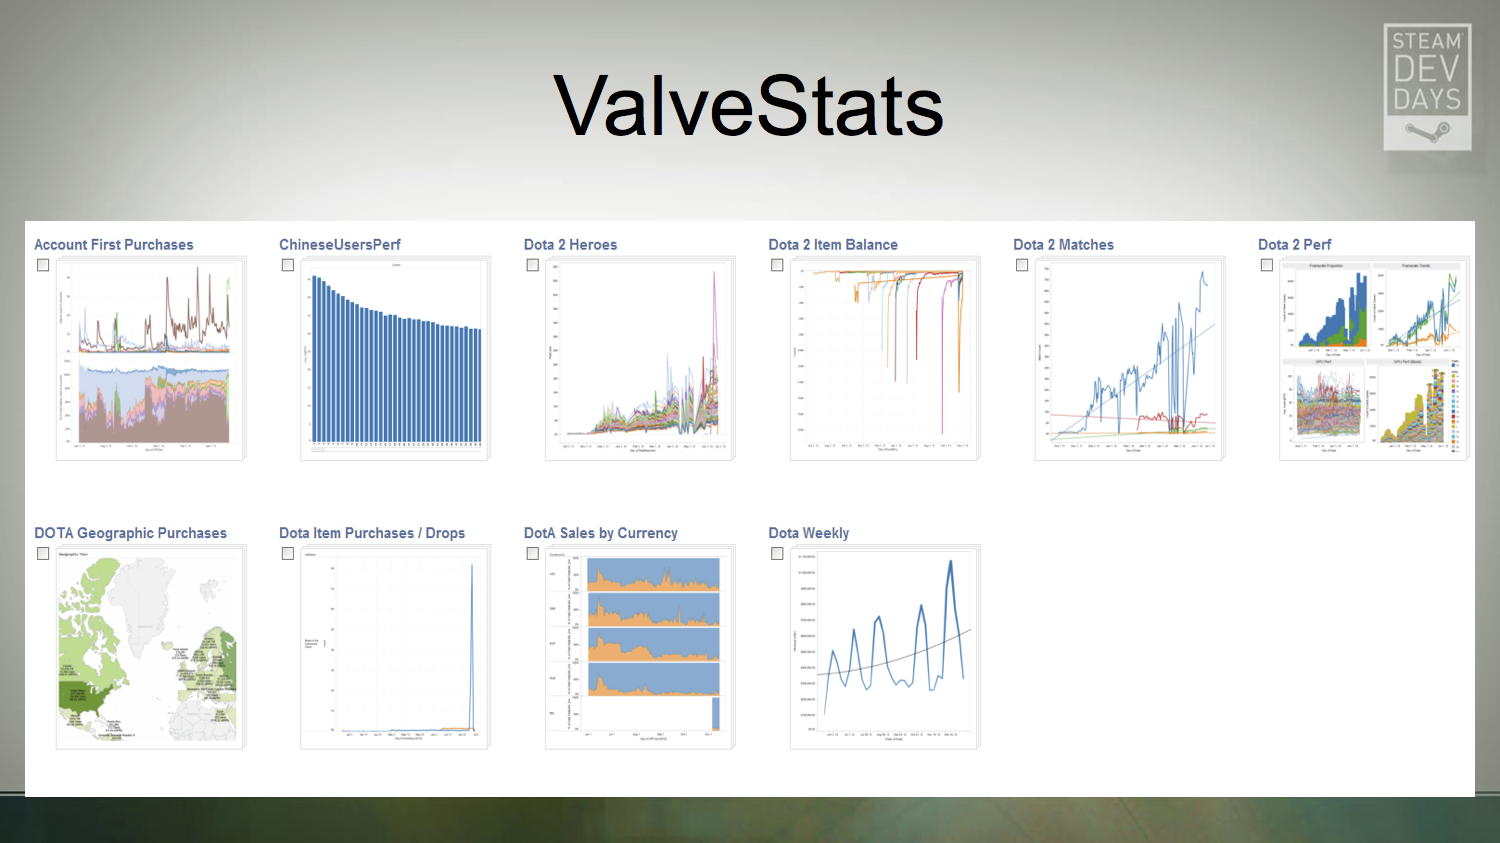
\includegraphics[width=\paperwidth]{valve_stats}
		};
	\end{tikzpicture}
\end{frame}

\begin{frame}{Player deaths in Team Fortress 2}
	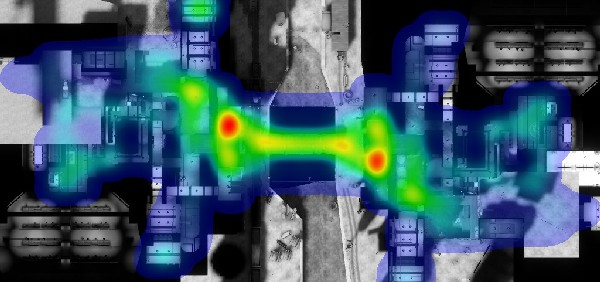
\includegraphics[width=\textwidth]{heatmap_tf2}
\end{frame}

\begin{frame}{Weapon fire locations in CS:GO}
	\begin{center}
		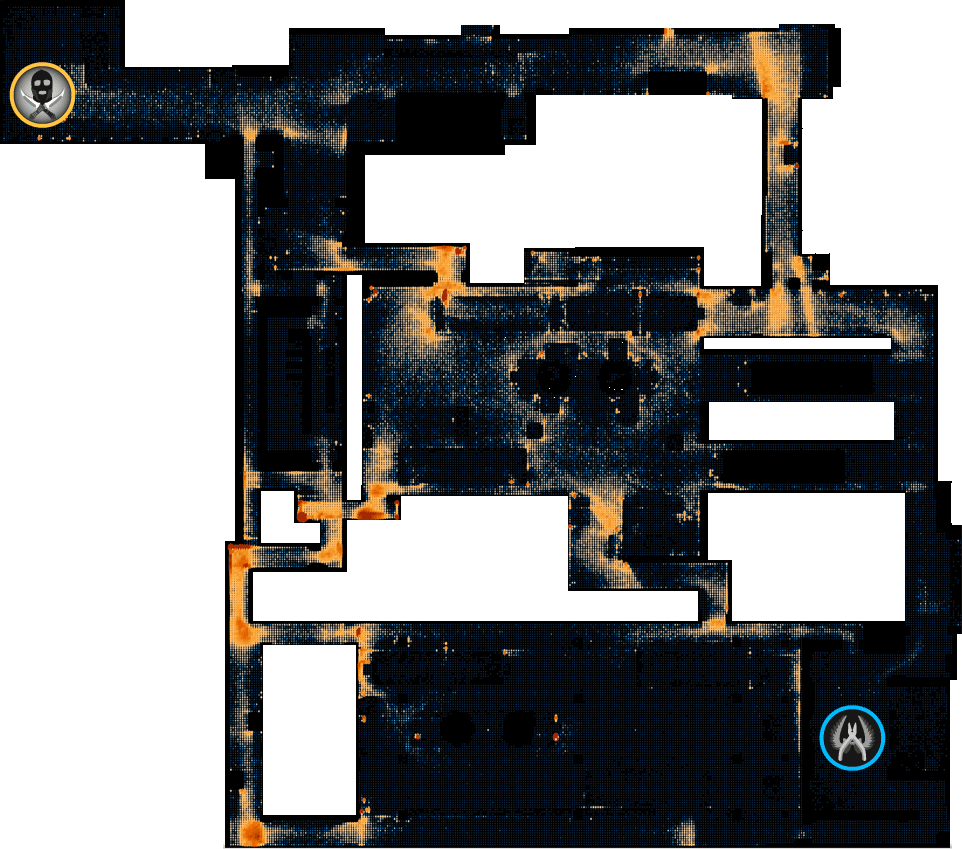
\includegraphics[height=0.8\textheight]{heatmap_csgo}
	\end{center}
\end{frame}

\begin{frame}{Data visualisation}
	\begin{itemize}
		\pause\item Humans are good at seeing \textbf{patterns}
		\pause\item Good data visualisation can help to spot patterns
		\pause\item ... However this should be followed up by proper statistical analysis!
	\end{itemize}
\end{frame}

\part{Psychology}
\frame{\partpage}

\begin{frame}
	\begin{center}
		
\includegraphics[width=0.4\textwidth]{riot_logo}
		
		\url{http://gdcvault.com/play/1017940/The-Science-Behind-Shaping-Player}
		
		\url{https://backchannel.com/inside-the-largest-virtual-psychology-lab-in-the-world-7c0d2c43cda5\#.e63is9hkl}
	\end{center}
\end{frame}

\begin{frame}{Priming}
	\begin{itemize}
		\pause\item How do you pronounce this word: S - H - O - P?
		\pause\item What do you do at a green traffic light?
	\end{itemize}
\end{frame}

\begin{frame}{A/B testing}
	\begin{itemize}
		\pause\item Push \textbf{different versions} of your game to different groups of players
		\pause\item Measure over different groups to compare effects of changes
		\pause\item Not restricted to two versions
	\end{itemize}
\end{frame}

\begin{frame}{Priming in League of Legends}
	\begin{itemize}
		\pause\item \textbf{Hint text} on loading screen and/or in-game
		\pause\item ``X\% of players punished by the Tribunal improve their behaviour and are never punished again''
		\pause\item Led to a \textbf{6\% decrease} in verbal abuse and offensive language
	\end{itemize}
\end{frame}

{\setbeamercolor{background canvas}{bg=black}

\begin{frame}{Priming in League of Legends}
	\begin{itemize}
		\pause\item ``Teammates perform worse if you harass them after a mistake''
		\pause\item $\to$ \textbf{No significant} impact
		\pause\item ``\textcolor{red}{Teammates perform worse if you harass them after a mistake}''
		\pause\item $\to$ \textbf{11\% decrease} in offensive language
	\end{itemize}
\end{frame}

\begin{frame}{Priming in League of Legends}
	\begin{itemize}
		\pause\item ``\textcolor{red}{Players who cooperate with their teammates win $X$\% more games}''
		\pause\item $\to$ \textbf{No significant} impact
		\pause\item ``\textcolor{blue!50}{Players who cooperate with their teammates win $X$\% more games}''
		\pause\item $\to$ \textbf{6\% decrease} in offensive language
	\end{itemize}
\end{frame}

\begin{frame}{Priming in League of Legends}
	\begin{itemize}
		\pause\item ``\textcolor{red}{Who will be the most sportsmanlike player in the game?}''
		\pause\item $\to$ \textbf{15\% increase} in offensive language
	\end{itemize}
\end{frame}

} % end of black bg

\begin{frame}{Games as experiments}
	\begin{itemize}
		\pause\item These experiments would be difficult to do in the lab
		\pause\item ... and impossible at this scale (\textbf{millions} of participants)
		\pause\item Results have a \textbf{measurable positive impact} on player experience
	\end{itemize}
\end{frame}


\part{Monetisation}
\frame{\partpage}

\begin{frame}
	\begin{tikzpicture}[remember picture, overlay]
		\node[at=(current page.center)] {
			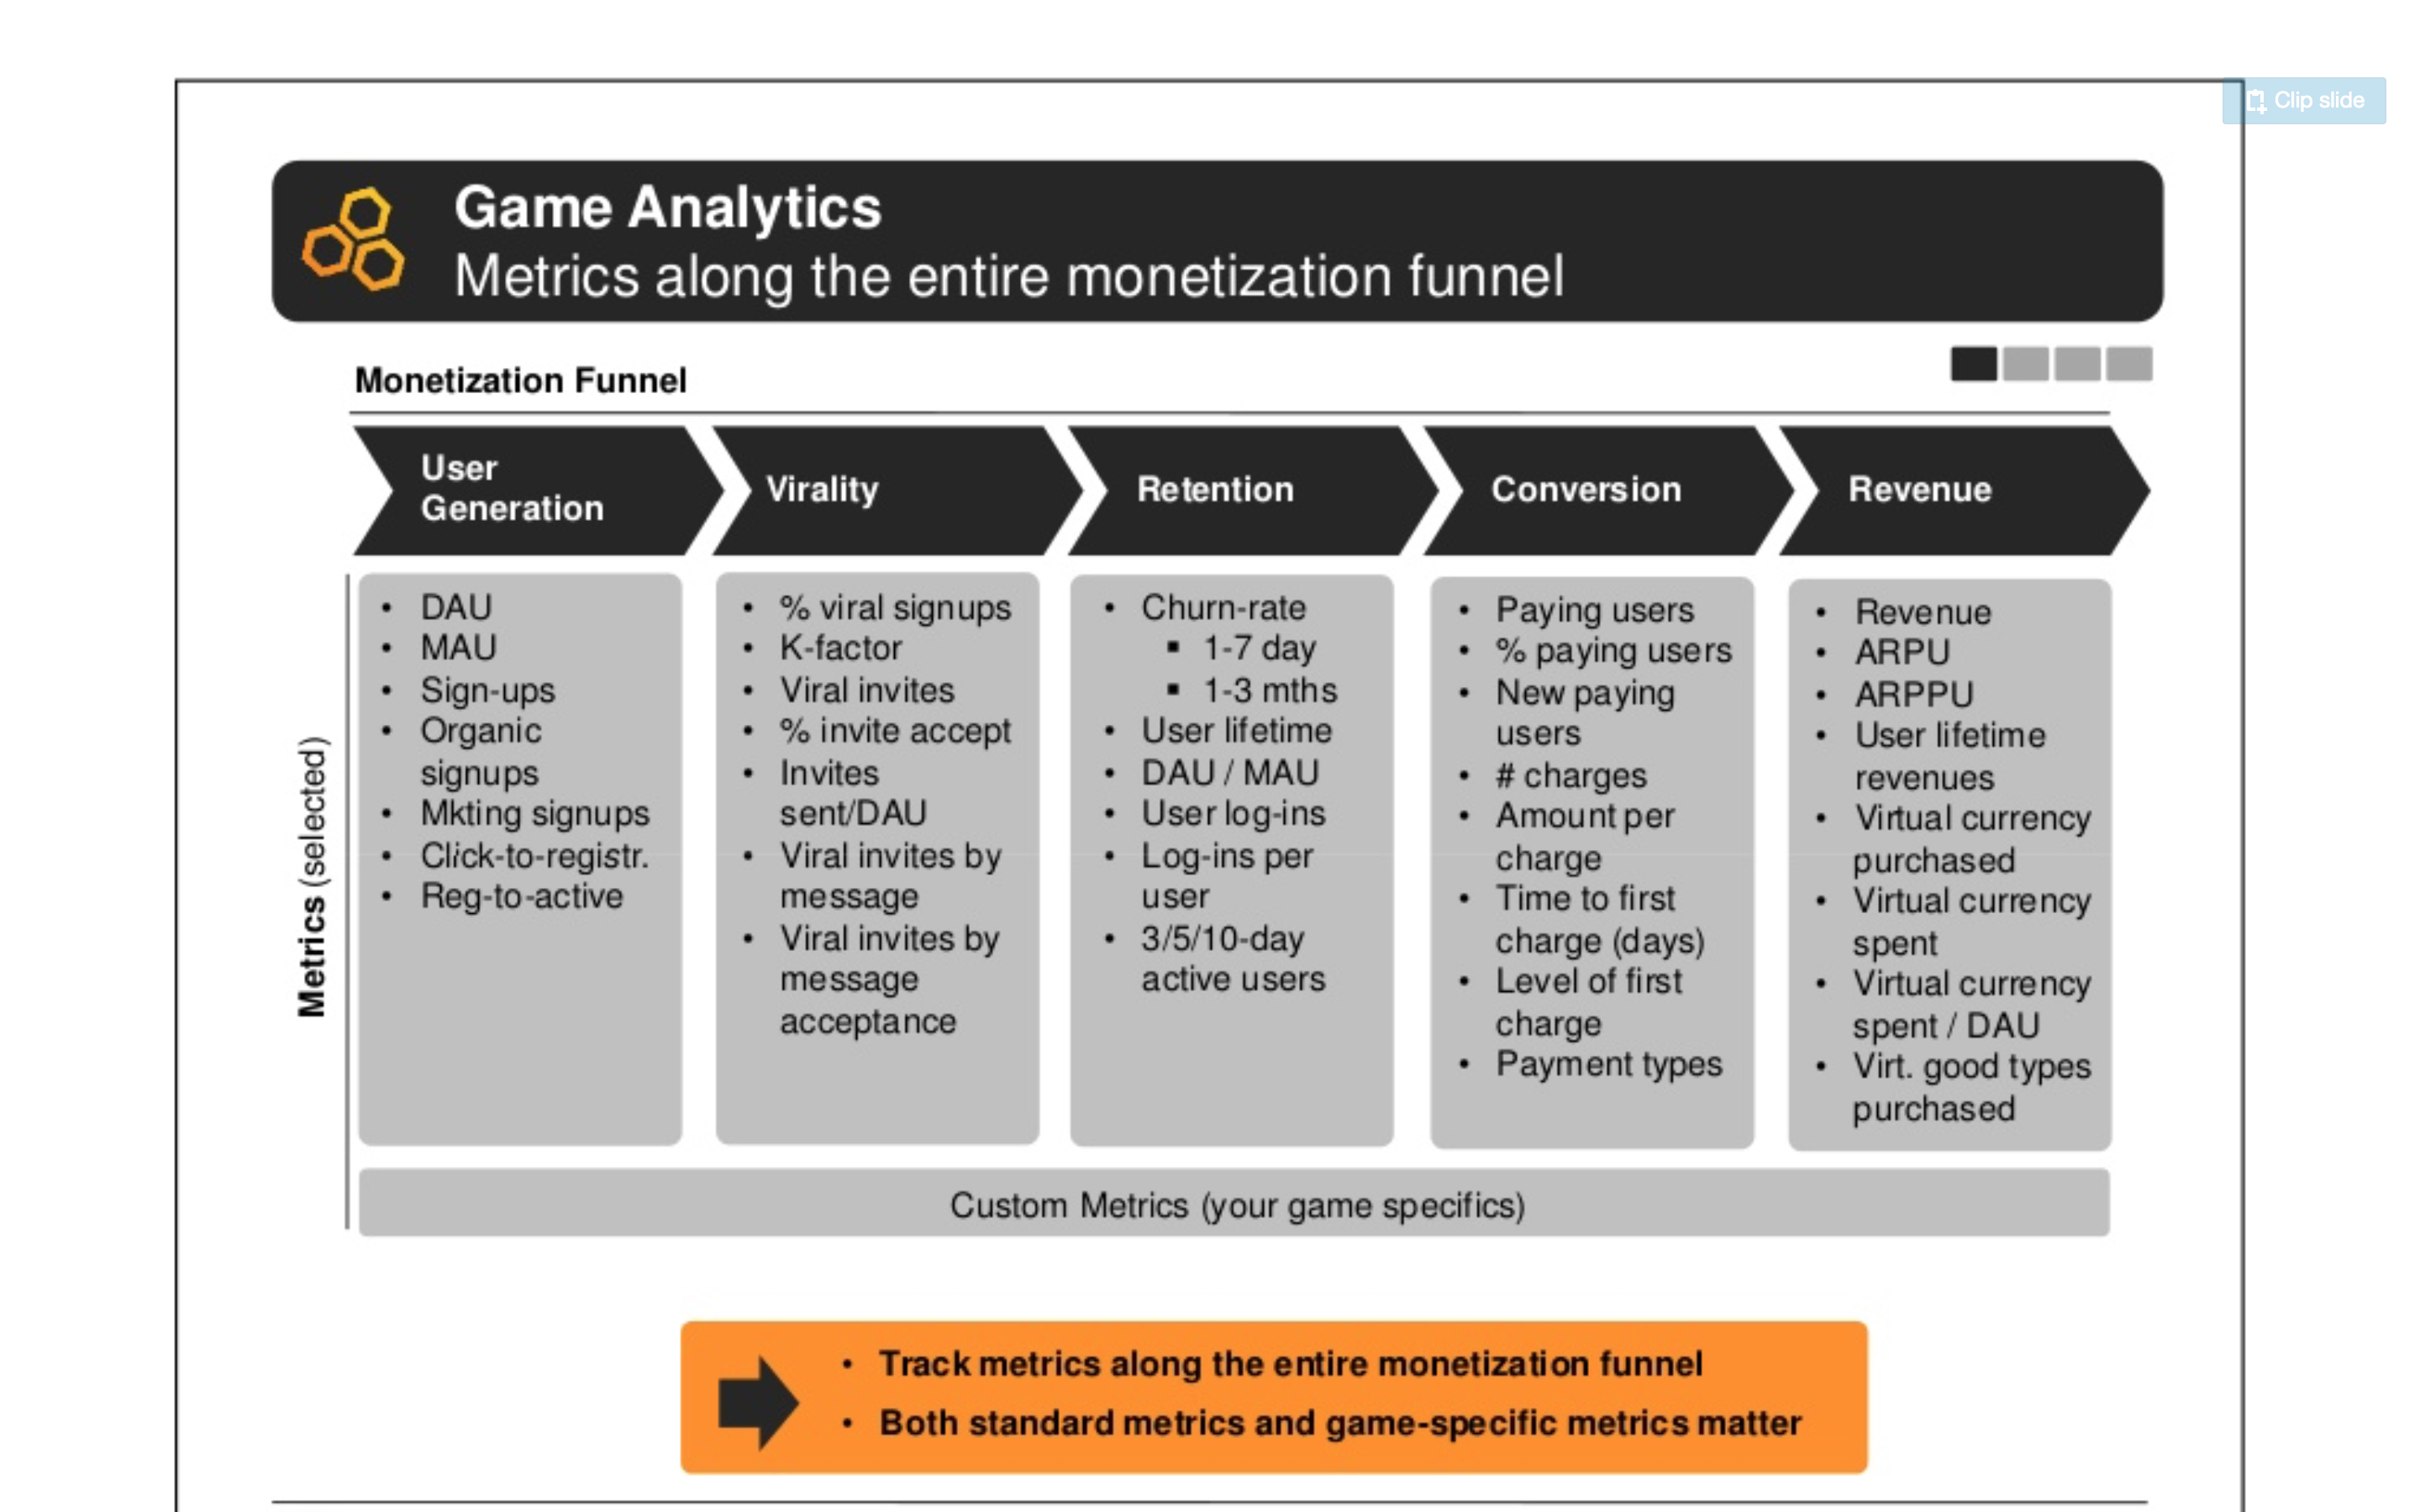
\includegraphics[width=\paperwidth]{f2p_metrics}
		};
	\end{tikzpicture}
\end{frame}

\begin{frame}{Metrics of monetisation}
	\begin{itemize}
		\pause\item Successful \textbf{free-to-play} games (particularly on mobile) are driven by analytics
		\pause\item Drawing heavily on metrics developed by \textbf{marketing} and \textbf{advertising} industries
		\pause\item Negative view:
			\begin{itemize}
				\pause\item Optimising profitability at the expense of player experience
				\pause\item Geared towards squeezing as much money out of ``whales'' as possible
			\end{itemize}
		\pause\item Positive view:
			\begin{itemize}
				\pause\item Enables new business models, e.g.\ games-as-a-service
				\pause\item Can enhance player experience if done carefully
			\end{itemize}
	\end{itemize}
\end{frame}


% case study 1: Valve https://andersdrachen.com/2014/02/14/mike-ambinder-on-valves-journey-towards-becoming-data-driven/
% case study 2: LoL https://backchannel.com/inside-the-largest-virtual-psychology-lab-in-the-world-7c0d2c43cda5#.e63is9hkl
% case study 3: f2p https://www.slideshare.net/TomSente/game-monetization-analytics-how-to-use-your-game-metrics-effectively

\part{Ethics of analytics}
\frame{\partpage}

\begin{frame}
	\begin{columns}
		\begin{column}{0.48\textwidth}
			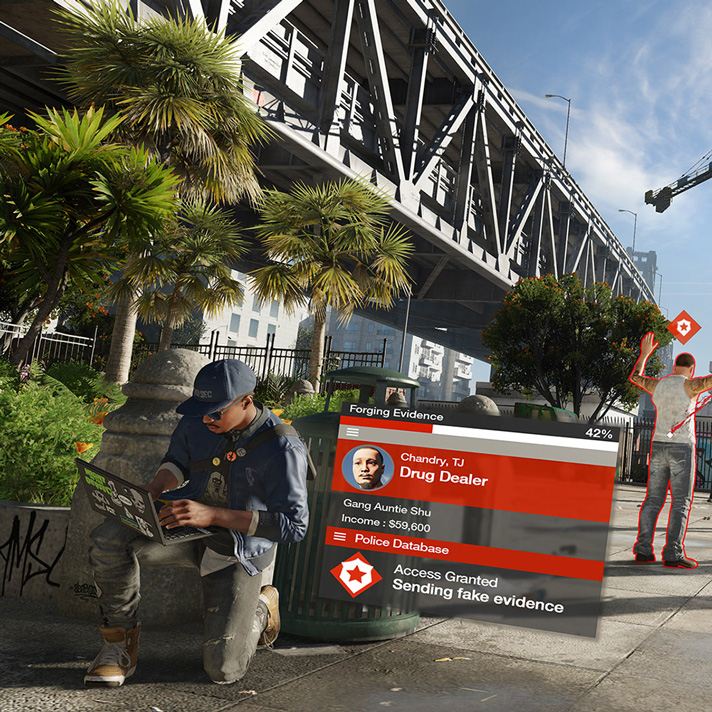
\includegraphics[width=\textwidth]{watch_dogs_2}
		\end{column}
		\pause
		\begin{column}{0.48\textwidth}
			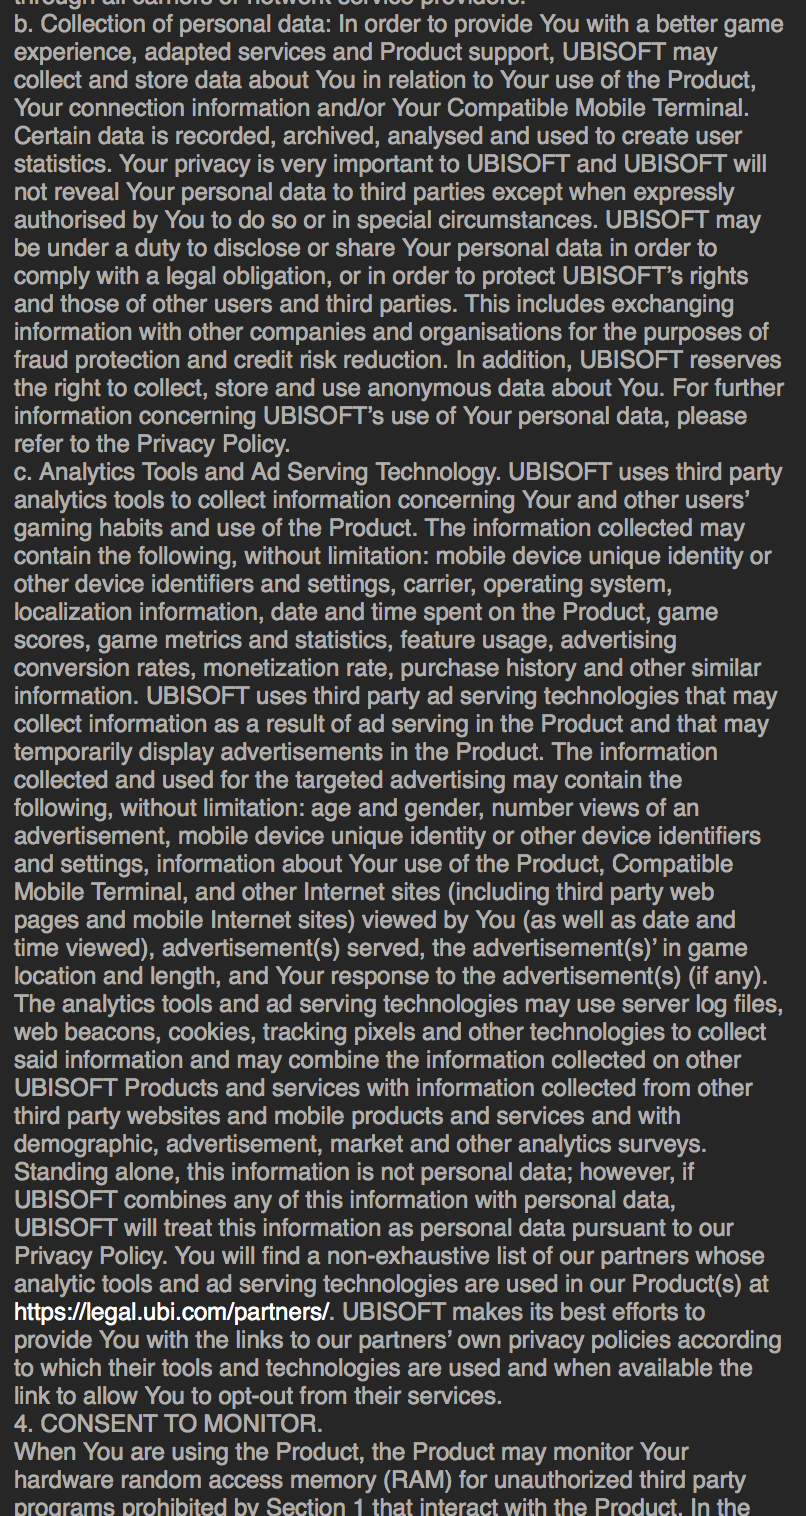
\includegraphics[height=\textheight]{watch_dogs_2_eula}
		\end{column}
	\end{columns}
\end{frame}

\begin{frame}{Ethical considerations}
	\begin{itemize}
		\pause\item Are you breaching your players' \textbf{privacy}?
		\pause\item Is it right to \textbf{experiment} on your players?
		\pause\item Is it right to \textbf{manipulate} your players' behaviour?
		\pause\item Are you deliberately adding \textbf{addictive} qualities to your game?
		\pause\item Is the above justified if it improves the player \textbf{experience}?
		\pause\item What if it improves your \textbf{profits} instead / as well?
	\end{itemize}
\end{frame}

\begin{frame}{Legal considerations}
	\begin{itemize}
		\pause\item \textbf{NB: this slide is for education only and does NOT constitute legal advice!}
        \pause\item Legislation such as the \textbf{General Data Protection Regulation (GDPR)} and the
            \textbf{Data Protection Act}
		\pause\item Covers \textbf{personal data}: any data that can be used to identify a living individual
			\begin{itemize}
				\pause\item Name, phone number, email address, IP address, social media ID, ...
			\end{itemize}
		\pause\item Covers the \textbf{processing} (including storage) of personal data
		\pause\item The data processor has certain \textbf{responsibilities}
		\pause\item The data subject has certain \textbf{rights}
		\pause\item Not complying can be a \textbf{civil and/or criminal offence}
	\end{itemize}
\end{frame}


\begin{frame}{Conclusion}
	\begin{itemize}
		\pause\item Analytics can be seen as \textbf{large-scale playtesting}
		\pause\item Allows a \textbf{scientific} approach to game design decisions
		\pause\item Allows a \textbf{scientific} approach to business decisions
	\end{itemize}
\end{frame}

\begin{frame}
	\begin{center}
		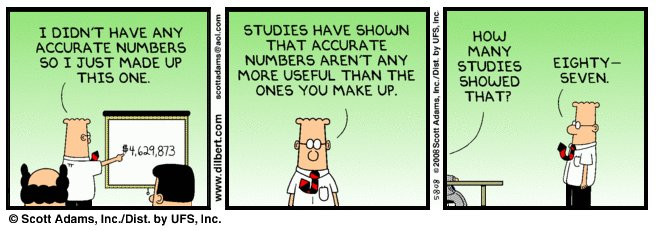
\includegraphics[width=\textwidth]{dilbert}
	\end{center}
\end{frame}

\end{document}
